\section{Hardware}

\textbf{Johnson Motor:} In this project, the Johnson motor plays a crucial role in the mobility and navigation system of the robot. As a geared DC motor known for its high torque and moderate speed, the Johnson motor is ideal for driving the wheels of the line-following robot, especially in environments such as hospital wards or hostels where smooth and controlled movement is essential. Its robust build and metal gearbox allow it to handle the weight of the robot's three compartments, including the lower section for motion and trays, the middle for storage, and the top for pill dispensing. The motor’s torque ensures that the robot can move efficiently even while carrying a moderate load, without stalling or losing stability. Since the robot needs to follow a pre-defined path using line-following sensors, the Johnson motor provides the precision required to maneuver accurately around corners, stop at designated points like patient beds, and resume movement seamlessly. Its compatibility with motor driver modules like the L298N allows for easy integration into the robot’s electronic control system, enabling direction and speed control through microcontrollers or the Raspberry Pi. Additionally, Johnson motors operate at low voltage (typically 6V to 12V), which aligns well with the power requirements of compact, battery-operated robots.

\begin{figure}[htbp!]
\centering
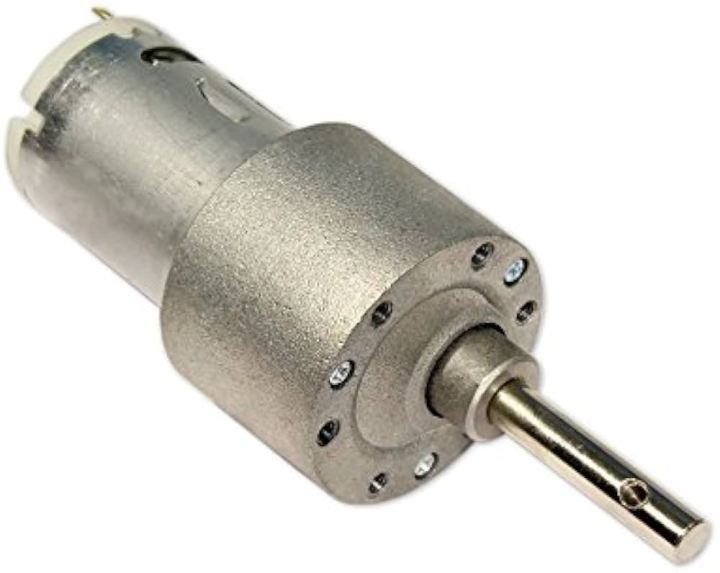
\includegraphics[width=0.5\textwidth]{images/3.1.jpg}
\caption{\textbf{Johnson Motor}}
\label{fig:3.1}
\end{figure}

\vspace{1.5\baselineskip} % Adds 1.5 line spaces before next section

\textbf{Raspberry pi 4:} In this project, the Raspberry Pi 4 with 4GB RAM serves as the central processing unit for managing high-level tasks such as patient recognition, time-based scheduling, and controlling the pill dispensing mechanism. With its quad-core processor and sufficient RAM, the Raspberry Pi 4 efficiently handles image processing tasks using a connected camera module to recognize patients either through facial recognition or QR code scanning. It also maintains an internal clock (with or without an external RTC module) to ensure pills are dispensed accurately according to schedule. The 4GB RAM allows for smooth multitasking, such as running Python scripts for motor control, image recognition algorithms, and logging data, all at once without lag. The Raspberry Pi also communicates with external hardware like servo motors for pill dispensing and the motor driver for controlling movement if necessary. Additionally, its GPIO pins can be used to interface with sensors and control systems, while built-in Wi-Fi and Bluetooth allow for wireless updates, alerts, or remote monitoring through a mobile app or web interface. In summary, the Raspberry Pi 4 (4GB) provides the computing power and flexibility needed to control smart operations in the top compartment of the robot, making it an intelligent and autonomous medical assistant.

\begin{figure}[htbp!]
\centering
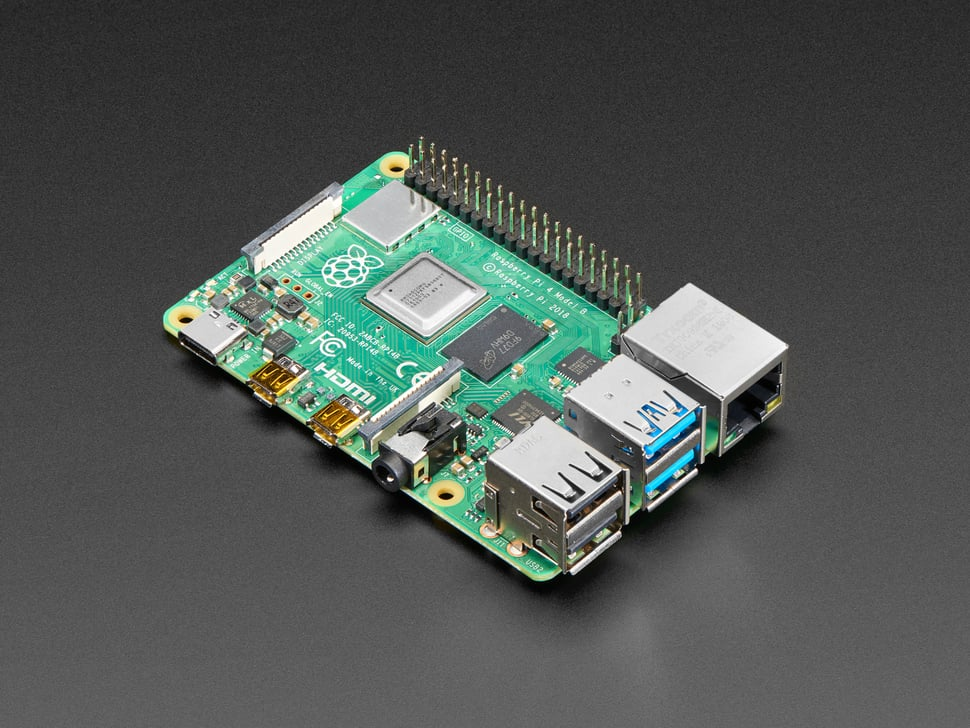
\includegraphics[width=0.5\textwidth]{images/fig3.2.jpg}
\caption{\textbf{Raspberry pi 4}}
\label{fig:3.2}
\end{figure}

\vspace{1.5\baselineskip} % Adds 1.5 line spaces before next section

\textbf{Arduino UNO}: In this project, the Arduino Uno plays a critical role as the microcontroller responsible for handling low-level hardware operations, particularly in the bottom compartment of the robot. It is used to read input from IR sensors for line-following, control the Johnson motors via a motor driver (such as the L298N), and manage other components like buzzers or LEDs for alerts. The Arduino Uno is well-suited for this task due to its simplicity, reliability, and ease of programming. With 14 digital I/O pins and 6 analog inputs, it can easily interface with multiple IR sensors, motors, and additional modules if needed. It operates on 5V logic, making it compatible with most common robotic components. The Arduino continuously reads sensor data and processes it in real time to make decisions about movement—like turning left or right, stopping at specific points, or correcting its path. It can be programmed using the Arduino IDE with simple C/C++ code, making development and debugging accessible even for beginners. In this project, the Arduino Uno ensures stable and responsive control over the robot’s motion system, allowing the Raspberry Pi to focus on higher-level tasks such as patient recognition and pill dispensing in the upper compartment.

\begin{figure}[htbp!]
\centering
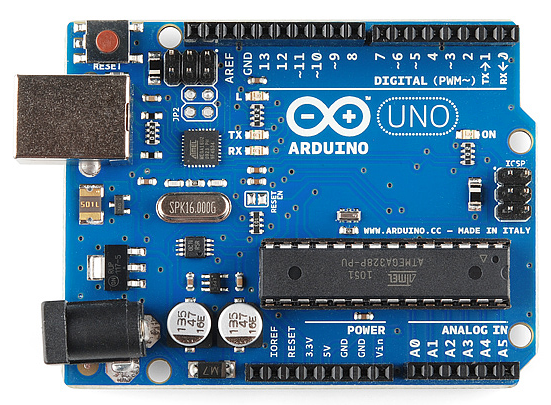
\includegraphics[width=0.5\textwidth]{images/fig3.3.png}
\caption{\textbf{Arduino UNO}}
\label{fig:3.3}
\end{figure}

\vspace{1.5\baselineskip} % Adds 1.5 line spaces before next section

\textbf{IR array Sensors: }In this project, the IR (Infrared) sensor is a key component used in the bottom compartment of the robot to enable line-following capability. IR sensors work by emitting infrared light and detecting its reflection from surfaces. When placed near the ground, they can distinguish between dark lines (which absorb more light) and lighter backgrounds (which reflect more light). By strategically placing multiple IR sensors on the bottom of the robot, the system can detect and follow a black line on a white surface or vice versa. This allows the robot to navigate predetermined paths accurately within structured environments such as hospital wards or hostels. The data from the IR sensors is continuously read by a microcontroller or Raspberry Pi, which then adjusts the motor speed and direction to keep the robot on track. This sensor-based navigation is simple, reliable, and cost-effective, requiring minimal setup while offering precise control. Additionally, IR sensors can help detect endpoints or junctions along the path by identifying sudden changes in surface color. In this way, the IR sensors play a vital role in ensuring the robot moves autonomously and accurately between bed positions for timely medicine delivery, enhancing the overall effectiveness of the system.

\begin{figure}[htbp!]
\centering
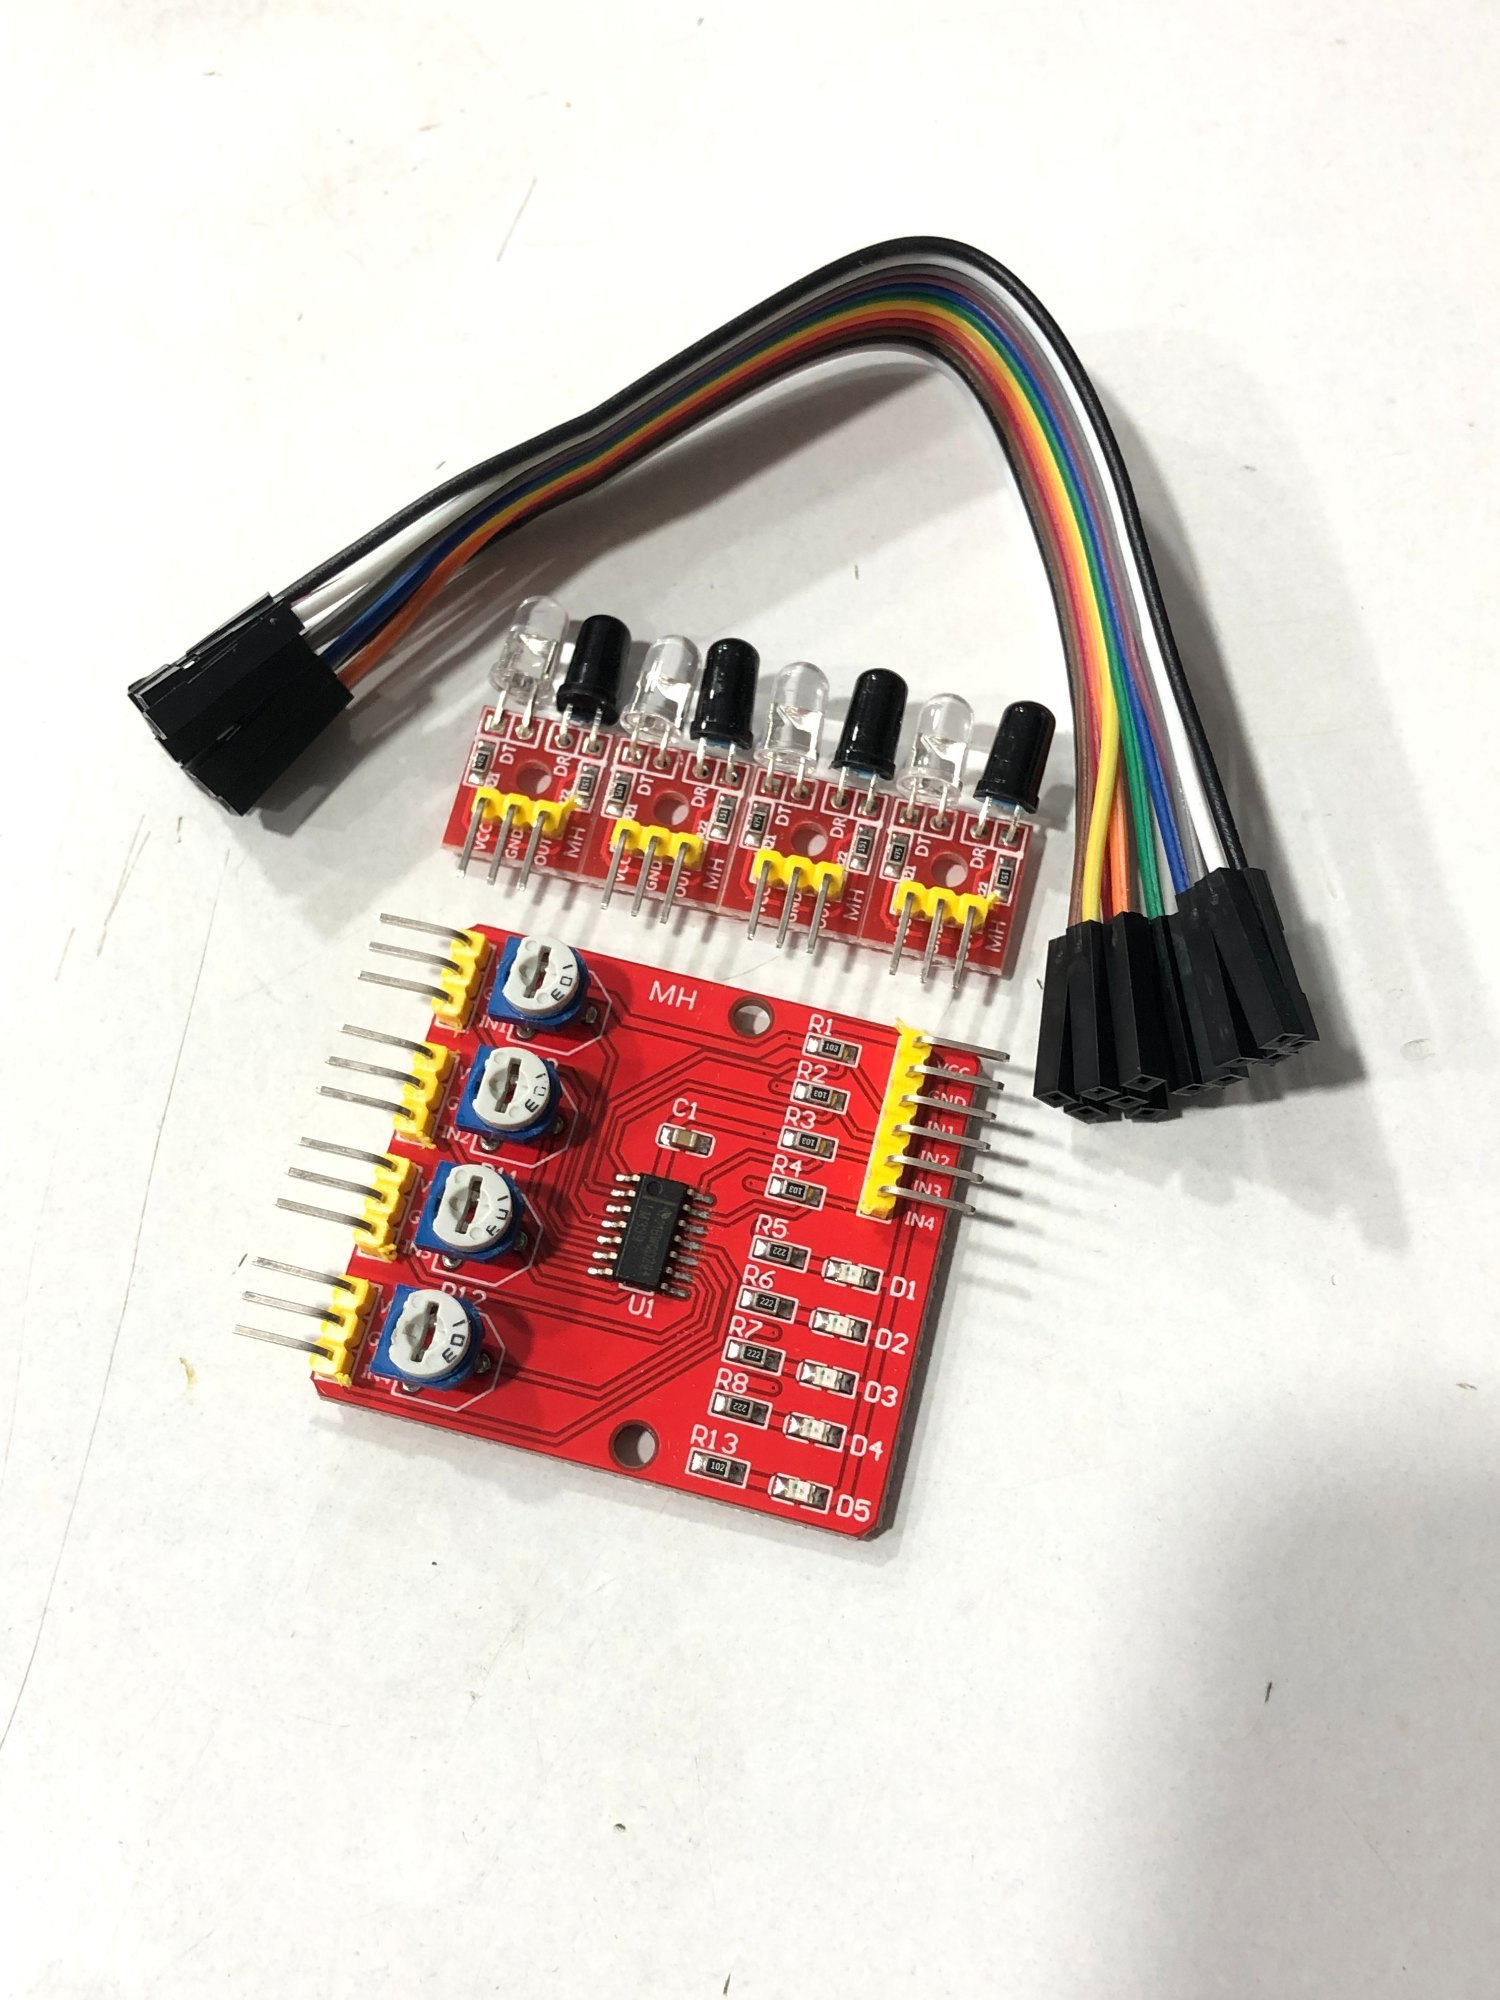
\includegraphics[width=0.5\textwidth]{images/3.4.jpg}
\caption{\textbf{IR array Sensors}}
\label{fig:3.4}
\end{figure}

\vspace{1.5\baselineskip} % Adds 1.5 line spaces before next section

\textbf{Metal Gear Servo: }In this project, the Metal Gear Servo MG996R is used in the top compartment to control the pill dispensing mechanism. This servo motor is known for its high torque, durability, and precision, making it ideal for applications requiring accurate and repeated movements. The MG996R operates using pulse-width modulation (PWM), allowing it to rotate to specific angles—typically between 0° and 180°. In the pill dispenser, the servo can be programmed to rotate a certain angle to open a slot, release a specific dose of medication, and then return to its original position. Its metal gear construction ensures strength and reliability, even under continuous or repeated use, which is essential in a healthcare setting where precision and consistency are critical. The servo is controlled by the Raspberry Pi or Arduino through a PWM signal, making integration into the system straightforward. It operates on 5V and can be powered from the same supply used for other components. With its ability to handle moderate mechanical loads and provide precise control, the MG996R ensures that pills are dispensed accurately according to the patient’s schedule. This makes it a key component in automating the medicine delivery process in your smart healthcare robot.

\begin{figure}[htbp!]
\centering
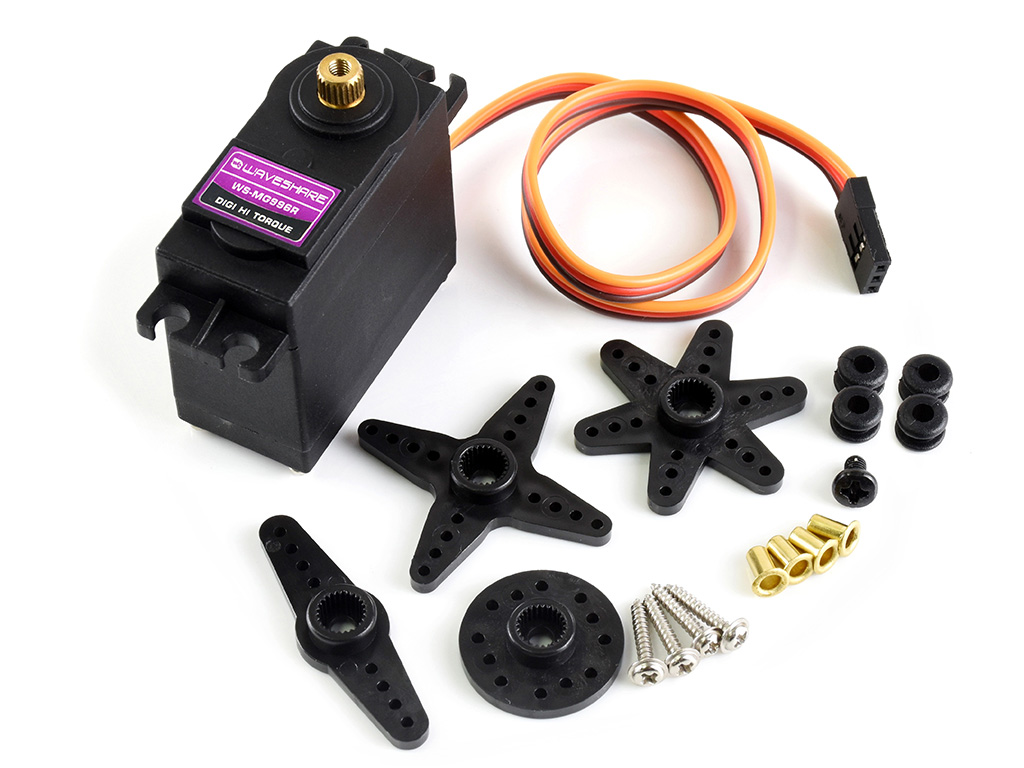
\includegraphics[width=0.5\textwidth]{images/3.5.jpg}
\caption{\textbf{Metal Gear Servo MG996R}}
\label{fig:3.5}
\end{figure}

\section{Software}

\textbf{Arduino IDE:} The Arduino Integrated Development Environment (IDE) is used to program the Arduino microcontroller responsible for real-time control of motors, sensors, and actuators. Written in C/C++, the code implements PID algorithms for accurate line following, triggers pill dispensing via servo motors, and reads data from modules such as IR sensors, UHF RFID readers, and ultrasonic sensors. Libraries like \texttt{Servo.h}, \texttt{Wire.h}, and \texttt{SoftwareSerial.h} simplify hardware interactions. Serial communication with the Raspberry Pi enables synchronous operation and system-level decision-making. The IDE’s Serial Monitor is invaluable for debugging sensor readings and validating motor responses, supporting firmware-level coordination for the robot’s motion and dispensing tasks.

\vspace{0.5em}

\textbf{Raspberry Pi \& Camera Module:} The Raspberry Pi 4 Model B, paired with the Raspberry Pi Camera V2 (NoIR), serves as the high-level processing unit of the system. It runs Python scripts for facial recognition using OpenCV and manages scheduled pill dispensing through a timetable system. Sensor feedback and motor status are received from the Arduino via UART serial communication, enabling dynamic coordination based on environmental inputs and patient recognition. The onboard real-time clock (RTC, optional) ensures precise execution of time-based actions. Captured facial data is matched with a patient database to ensure accurate medication delivery. A local SQLite or CSV-based logging system maintains records for real-time auditing and system monitoring.

\vspace{0.5em}

\textbf{Blender:} Blender, while not central in the current phase, may be employed for visual prototyping, robot path planning simulation, and 3D modeling of the robot’s compartments—including sliding tray mechanisms and modular structures. Using Blender’s Python API (\texttt{bpy}), simulations of compartment stacking and CAD-like assemblies can be rendered, providing a clear indication of hardware integration points and assisting in early-stage design validation.

\vspace{0.5em}

\textbf{Python Middleware:} Python acts as a critical middleware layer, bridging hardware and software. With \texttt{PySerial}, it decodes raw Arduino sensor data (e.g., accelerometer, gyroscope) into actionable gesture commands. These commands can trigger Blender animations via the \texttt{bpy} API, mapping real-world motions to virtual actions like grabbing or rotating objects. Python scripts also handle sensor calibration, noise filtering, and data normalization, enhancing interaction accuracy. This versatile setup supports rapid prototyping—from adjusting sensor thresholds to automating simulation updates—ensuring seamless real-time communication between hardware and virtual environments.



%\section{Dataset}
%\lipsum[4-8]
